\documentclass[Ex4_Zusammenfassung.tex]{subfiles}

\begin{document}

\section{Kernfusion}
\textbf{von \michi und \anton} \newline
2 Kerne verschmelzen zu einem schwereren Kern. \newline
\textbf{Vorraussetzung:} Genug kin. Energie vorhanden, um Coulomb-Barriere zu überwinden. \newline
Nach Überwindung der Coulomb-Barriere setzt die starke Kernkraft ein. Hierfür ist allerdings eine hohe Temperatur nötig ($\braket{E_{kin}} = \frac{3}{2} \ k_B \ T $) \newline
Um die Coulomb-Barriere zu überwinden nutzt das Teilchen den Tunneleffekt. (Abb.11.8)
\begin{figure}[H]
\centering
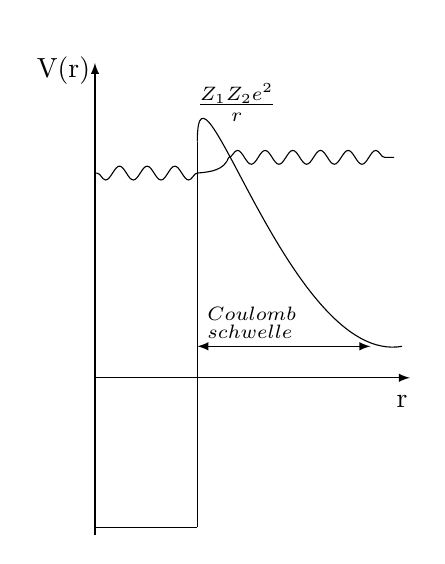
\begin{tikzpicture}
\draw [->,>= latex, thin] (0,0) -- (4,0);
\draw [->,>= latex, thin] (0,-2) -- (0,4);
\draw (0,-1.9) -- (1.3,-1.9);
\draw (1.3,-1.9) -- (1.3,3);
\draw (1.3,3) to [out=90,in=190] (3.9,0.4);
\draw [<->,>= latex,thin] (1.3,0.4) -- (3.5,0.4);
\draw [decorate,decoration=snake] (1.7,2.8) -- (3.8,2.8);
\draw (1.3,2.6) to [out=5,in=250] (1.7,2.8);
\draw [decorate,decoration=snake] (1.3,2.6) -- (0,2.6);


\node at (-0.4,3.9) {V(r)};
\node at (3.9,-0.3) {r};
\node at (2.0,0.7) {$^{Coulomb}_{schwelle}$};
\node at (1.8,3.5) {$\frac{Z_1 Z_2  e^2}{r}$};
\end{tikzpicture}
\caption{Coulombbarriere und Tunneleffekt}
\end{figure}
\textbf{Energiebilanz:} \newline
Eisen hat die maximale Bindungsenergie pro Massenzahl ($\nicefrac{E_B}{A}$). Somit setzt die Fusion zu kleinen oder gleich großen Kernen wie Eisen Energie frei. Bei größeren Kernen setzt die Spaltung dann Energie frei. \newline
Wie wichtig der Tunneleffekt für die Kernfusion ist zeigt sich am Beispiel der Sonne. Dort beträgt die mittlere Temperatur $T \approx 1.5 \cdot 10^7$ K.  Dies entspricht einer kinetischen Energie von $E_{kin} \approx 1$ keV. Aber für das Potential das überwinden werden muss gilt: 
\begin{equation}
V_{cb} (2H \rightarrow d + e^+ + \nu_{e}) = \frac{e^2}{r} \approx \frac{1.44 \  MeV fm}{1 \ fm} = 1.44 \ MeV \gg 1 \  keV
\end{equation}
Wobei als Abstand $r \approx 1$ fm angenommen wurde. Bei diesem Abstand dominiert die starke Wechselwirkung auf jeden Fall die Coulomb-Wechselwirkung (Sind gleich bei $r \approx 2.5$ fm), wodurch wir sicher sein können, dass das Teilchen im Kern bleibt. \newline
Man sieht anhand des Vergleichs dieser Energien, dass zur Kernfusion auf jeden Fall der Tunneleffekt nötig ist.

\end{document}